%%%%%%%%%%%%%%%%%%%%%%%%%%%%%%%%%%%%%%%%%%%%%%%%%%%%%%%%%%%%%%%%%%%%%%%%%%%%%%%%
% ECE 285 -- Homework 01 report  (2-page NeurIPS format)
%
% Compile:   pdflatex HW01_report.tex
% Needs:     neurips_2025.sty                (in this directory)
%            results/figures/*.png           (produced by HW01.ipynb)
%
% Every number below was taken from the notebook run:
%   results/metrics_summary.json, results/training_history.csv,
%   results/fid_is_history.csv
%
% The text is deliberately terse to fit two pages. What is shown is exactly what
% the brief asks for: hyperparameters (Table 1), loss curves (Fig. 1), IS/FID
% (Table 2 and Fig. 2, right) and generated images (Fig. 2, left). The
% reconstruction and latent-interpolation panels live in the notebook.
%
% If it still overflows by a few lines, shrink the \includegraphics widths.
%%%%%%%%%%%%%%%%%%%%%%%%%%%%%%%%%%%%%%%%%%%%%%%%%%%%%%%%%%%%%%%%%%%%%%%%%%%%%%%%
\documentclass{article}

% [preprint] -> "Preprint." footer, no line numbers. Use [final] for camera-ready.
\usepackage[preprint]{neurips_2025}

\usepackage[utf8]{inputenc}
\usepackage[T1]{fontenc}
\usepackage{hyperref}
\usepackage{url}
\usepackage{booktabs}
\usepackage{amsfonts}
\usepackage{amsmath}
\usepackage{amssymb}
\usepackage{microtype}
\usepackage{graphicx}
\usepackage{caption}
\usepackage{float}          % provides [H]: place the float exactly here

\graphicspath{{results/figures/}}

% Every float uses [H], so each figure/table lands immediately after the
% paragraph that first refers to it, never at the top of an earlier page.
\floatplacement{figure}{H}
\floatplacement{table}{H}

\captionsetup{font=small,labelfont=bf,skip=1pt}
\setlength{\textfloatsep}{5pt plus 2pt minus 2pt}
\setlength{\floatsep}{4pt plus 1pt minus 1pt}
\setlength{\intextsep}{6pt plus 1pt minus 1pt}
\setlength{\abovecaptionskip}{2pt}
\setlength{\belowcaptionskip}{0pt}
\setlength{\abovedisplayskip}{2pt plus 1pt}
\setlength{\belowdisplayskip}{2pt plus 1pt}

\title{ECE 285 Homework 01}

\author{%
  Youjie Xie \\
  TSN: 200232637 \\
  \texttt{yox005@ucsd.edu}
}

\begin{document}

\maketitle

\section{Method}

We implement a convolutional variational autoencoder (VAE) in PyTorch and train it on the Kaggle
\emph{Chest X-Ray Images (Pneumonia)} dataset to generate $64\times64$ chest radiographs. For
$x\in[0,1]^{1\times64\times64}$ we use a diagonal Gaussian posterior
$q_\phi(z\mid x)=\mathcal{N}(\mu_\phi(x),\operatorname{diag}\sigma_\phi^2(x))$, a factorised
Bernoulli likelihood and a standard normal prior. The $\beta$-weighted negative ELBO per image, in
nats, is
\begin{equation}
\mathcal{L}=\underbrace{\mathbb{E}_{q_\phi(z\mid x)}\!\left[-\log p_\theta(x\mid z)\right]}_{\text{BCE, summed over pixels}}
\;+\;\beta\,
\underbrace{D_{\mathrm{KL}}\!\left(q_\phi(z\mid x)\,\|\,\mathcal{N}(0,I)\right)}_{\text{closed form}},
\qquad z=\mu_\phi(x)+\sigma_\phi(x)\odot\epsilon,
\end{equation}
where $D_{\mathrm{KL}}=-\tfrac12\sum_{j}(1+\log\sigma_j^2-\mu_j^2-\sigma_j^2)$ and the BCE is summed
over pixels then divided by the batch size. Encoder and decoder are mirror-image convolutional
stacks of $\log_2 64-2=4$ stages ($4\times4$ kernels, stride 2, widths $32\to64\to128\to256$); two
linear heads give $(\mu,\log\sigma^2)\in\mathbb{R}^{128}$, and the decoder starts from
$\mathrm{FC}(128\to4096)$ and ends in a sigmoid. Batch-norm is omitted on the last encoder and first
decoder block. Training uses Adam with $10^{-3}$ cosine-decayed to $10^{-5}$ and gradient-norm
clipping at 5.0; $\beta$ ramps from 0 to 1 over 10 epochs, the standard remedy for early posterior
collapse. Table~\ref{tab:hparams} lists the configuration.

\begin{table}[H]
\centering
\small
\caption{Hyperparameter settings.}
\label{tab:hparams}
\begin{tabular}{@{}ll@{\hspace{1.2em}}ll@{}}
\toprule
image size & $64\times64$, 1 ch. & batch size & 64 \\
latent dim.\ $d$ & 128 & parameters & 2{,}955{,}905 \\
train / val / test & 4{,}694 / 522 / 624 & real reference & 512 images \\
optimiser & Adam ($0.9$, $0.999$) & learning rate & $10^{-3}\!\to\!10^{-5}$ \\
epochs & 50 (73 iters) & KL weight $\beta$ & $0\to1$ over 10 \\
grad.\ clipping & norm 5.0 & evaluation & every 5 epochs \\
\bottomrule
\end{tabular}
\end{table}

\section{Experimental setup}

The dataset holds 5{,}863 AP/PA radiographs, split officially into 5{,}216 / 16 / 624. The official
validation split has only 16 images, so we discard it and take a class-stratified 90/10 split of the
official training set (4{,}694 / 522, preserving the 74.3\,\% pneumonia prevalence). The 624-image
test set is never optimised on; a fixed 512-image subset is the \emph{real} reference. Images are
single-channel, resized to $64\times64$ with anti-aliased bilinear interpolation and scaled to
$[0,1]$ since the decoder predicts a Bernoulli mean; we apply \emph{no} horizontal flips because
chest radiographs are left/right asymmetric. For the Inception metrics a second pipeline produces
$3\times299\times299$ tensors from the \emph{original} JPEGs, giving a sharper reference than
upsampled crops.

\section{Results}

\paragraph{Training dynamics.} The loss (Fig.~\ref{fig:loss}) falls from 2728.97 to 2388.75 nats per
image --- 0.583 nats/pixel --- and still decays marginally at the end. Validation tracks training
closely (best 2362.41 at epoch 49), i.e.\ no overfitting, as expected for a 128-d bottleneck on
4{,}694 examples. The KL term \emph{contracts} from 112.38 to 24.08 nats while $\beta$ rises from 0.1
to 1.0, the intended $\beta$-VAE trade-off: reconstruction improves fast enough that the encoder can
approach the prior. The KL does not collapse, but 24.08 nats $\approx$ 34.7 bits over 128 dimensions
means few units are active --- which explains the blurriness, since the code carries ${\sim}$35 bits
about a 4{,}096-pixel image whose reconstruction term costs 3{,}412 bits.

\begin{figure}[H]
\centering
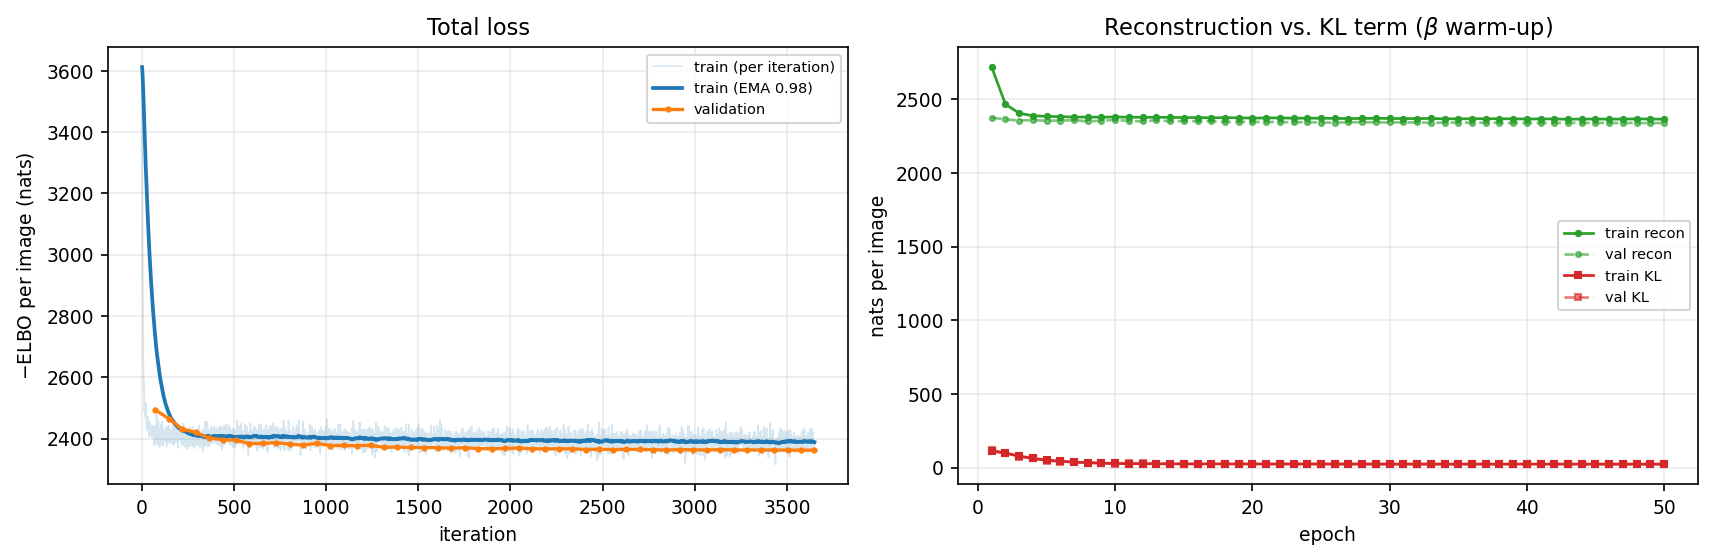
\includegraphics[width=0.88\linewidth]{loss_curves.png}
\caption{Training loss. \textbf{Left:} per-iteration loss (light) with its EMA (dark) and per-epoch
validation loss. \textbf{Right:} reconstruction and KL terms during the $\beta$ warm-up; KL
contracts from 112.4 to 24.1 nats while $\beta$ rises to 1.}
\label{fig:loss}
\end{figure}

\paragraph{Inception Score and FID.} Both metrics use an ImageNet-pretrained InceptionV3, following
the \texttt{pytorch-ignite} reference implementation: IS on its 1000-d softmax output and FID on its
2048-d pooling features, with inputs replicated to three channels and resized to $299\times299$ by
PIL bilinear interpolation. At the best checkpoint (epoch 45) the model reaches
\textbf{IS 1.618} and \textbf{FID 343.51}, against \textbf{2.289} and \textbf{66.30} for real images,
i.e.\ 71\,\% of the real IS (Table~\ref{tab:metrics}). Over epochs 5--50, IS climbs from 1.283 to a
plateau near 1.65 (peak 1.673 at epoch 45) while FID falls from 348.91 to 341.49 then rises to 344.39
at epoch 50. The two decouple late in training: IS keeps improving as samples become smoother and
more prototypical, whereas FID compares full feature covariances and saturates earlier. After epoch
30 FID has mean 343.3 and standard deviation 1.7, so the 0.35 margin of epoch 45 over epoch 30 is not
meaningful.

\begin{table}[H]
\centering
\small
\caption{FID and Inception Score on 512 held-out test images.}
\label{tab:metrics}
\begin{tabular}{@{}lcc@{}}
\toprule
 & Inception Score $\uparrow$ & FID $\downarrow$ \\
\midrule
Real test images (reference) & 2.289 & 66.30 \\
VAE, this work (epoch 45)    & 1.618 & 343.51 \\
\bottomrule
\end{tabular}
\end{table}

\paragraph{Generated images.} Prior samples (Fig.~\ref{fig:qual}, left) are unmistakably chest
radiographs: rib cage, lung fields, mediastinal column and diaphragm are present, with visible
variation in lung width, heart shadow and exposure. Missing is high-frequency detail --- ribs appear
as soft bands and no vascular markings survive. This is a property of the objective rather than of
the optimisation: under a Bernoulli likelihood the optimal prediction is the conditional mean of
each pixel given $z$, so averaging over residual uncertainty necessarily yields a smooth image.
Reconstructions recover global geometry at MSE 0.0034 while losing the same fine structure,
consistent with the 24-nat bottleneck.

\begin{figure}[H]
\centering
\begin{minipage}[b]{0.40\linewidth}
  \centering
  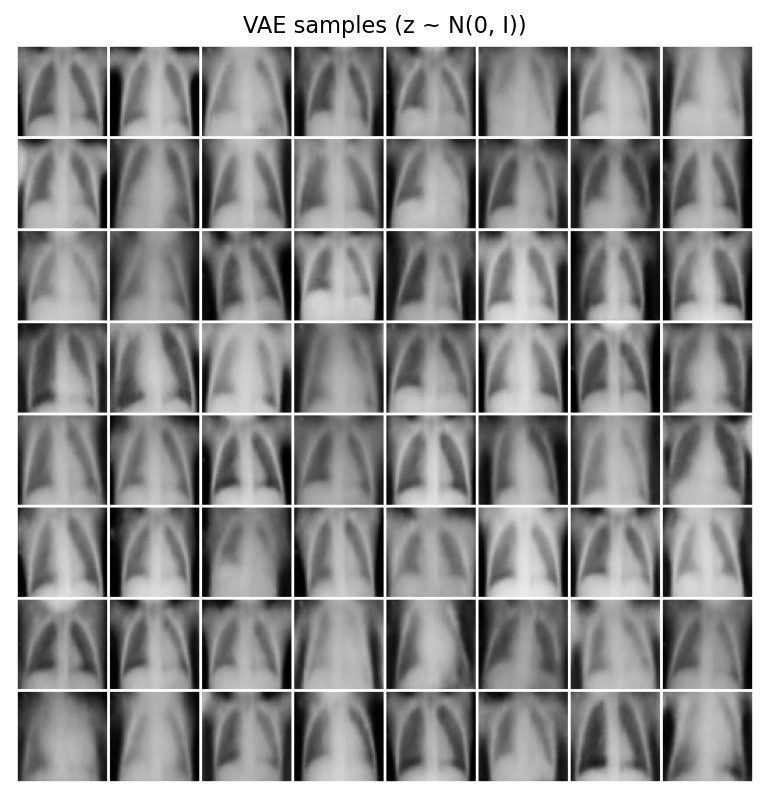
\includegraphics[width=\linewidth]{generated_samples.png}
\end{minipage}\hfill
\begin{minipage}[b]{0.56\linewidth}
  \centering
  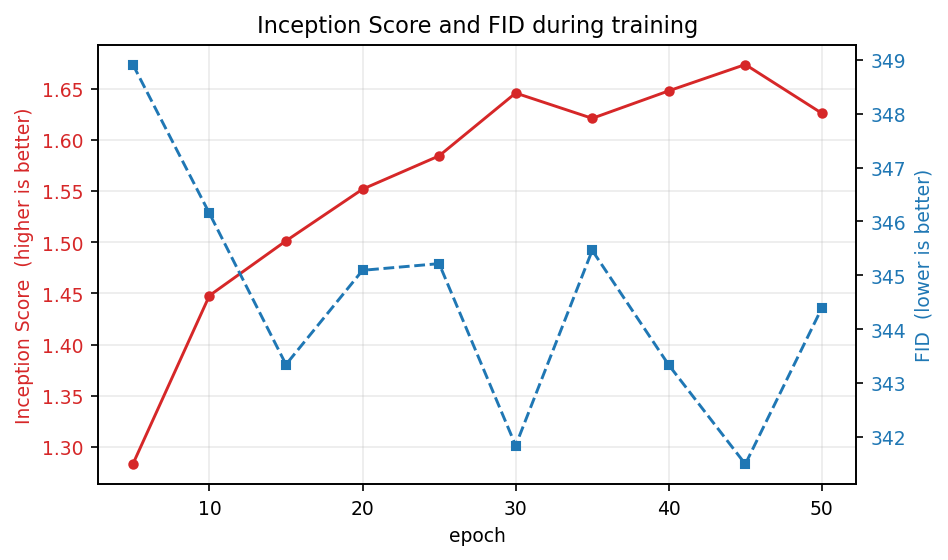
\includegraphics[width=\linewidth]{fid_is_curve.png}
\end{minipage}
\caption{\textbf{Left:} 64 samples from the prior $z\sim\mathcal{N}(0,I)$ at epoch 45.
\textbf{Right:} IS (higher better) and FID (lower better) every 5 epochs on the fixed 512-image
reference set.}
\label{fig:qual}
\end{figure}

\end{document}
